\documentclass{article}

\usepackage{fullpage}
\usepackage{titlesec}
\usepackage{parskip}
\usepackage{graphicx}
\usepackage{bold-extra}

\titleformat{\section}{\normalsize\bf}{}{0em}{}

\begin{document}

%\rightline{ }
\centerline{\large{\textbf{Distributed Multi-Heuristic A* (HAMSTAR)}}}
\centerline{Noam Brown, Aram Ebtekar, Yuzuko Nakamura}
\centerline{15-712 Fall 2014 Final Project Report}

\section{Abstract}

A* is a popular graph search algorithm used in many artificial intelligence applications. The original A* algorithm makes use of a single heuristic to prioritize exploration through a graph, but a variation on the algorithm known as multi-heuristic A* (MHA*) makes use of multiple heuristics to more quickly arrive at approximate solutions. For this project we implemented a distributed version of MHA*, with one process per heuristic. We show... [performance]
%TODO: Highlight important results

\section{Introduction}

Weighted A* is a simple, heuristic-based search algorithm used in artificial intelligence applications such as robotics and games. A heuristic function estimates the remaining distance from any state to the goal, thus guiding the search toward the goal. If the heuristic is \textbf{admissible}, meaning it never overestimates the true distance, then the solution is guaranteed to be optimal to within the weight factor. If it meets a stronger condition called \textbf{admissibility}, then no state needs to be expanded more than once.

Finding good heuristic functions is difficult, and moreover, finding an admissible heuristic function that is reasonably accurate over the entirety of the search space is often not practical. Multi-heuristic A* (MHA*) \cite{Aine14} is an alteration of the A* algorithm that allows the usage of a combination of multiple arbitrary heuristics to guide the search, while retaining the optimality bound of wA* provided that one consistent heuristic is used as an �anchor�. Where the shortcomings of each individual heuristic may result in local optima which trap the search, the ability to change heuristics can provide an escape.

In their work, Aine et al. propose two variants on MHA*: Independent Multi-Heuristic A* (IMHA*), where path cost and shortest path information are tracked separately for each heuristic, and Shared Multi-Heuristic A* (SMHA*), where shared knowledge of path cost and shortest path information are updated by all heuristics. SMHA* is the more effective of the two (explores the graph in a less repetitive manner and enables more co-operation between heuristics), but is more difficult to parallelize due to the amount of shared data.

For this project, we implemented a distributed version of this second variant, SMHA*.

\section{Relevant Work}

Our work is directly based off of Aine et al.'s original multi-heuristic anchored search \cite{Aine14} mentioned above. A parallelized version of the original A* algorithm was presented by Phillips et al. in \cite{Phillips14}. This method of parallelization makes inferences on when it's safe to expand multiple nodes in parallel, and in so doing maintains the approximate suboptimality guarantees of sequential wA*. This parallelization is dependent on the expansion operation being expensive enough to justify expanding multiple nodes in parallel, which may not be the case for all problems. By contrast, our method parallelizes the search process by constantly expanding multiple nodes chosen by different heuristics (instead of multiple nodes chosen by a single heuristic). As a result, our method differs from the previous in that, although nodes may be expanded multiple times by different machines, we do not require expansions to be slow.

\section{System Description}

\begin{figure}
\centering 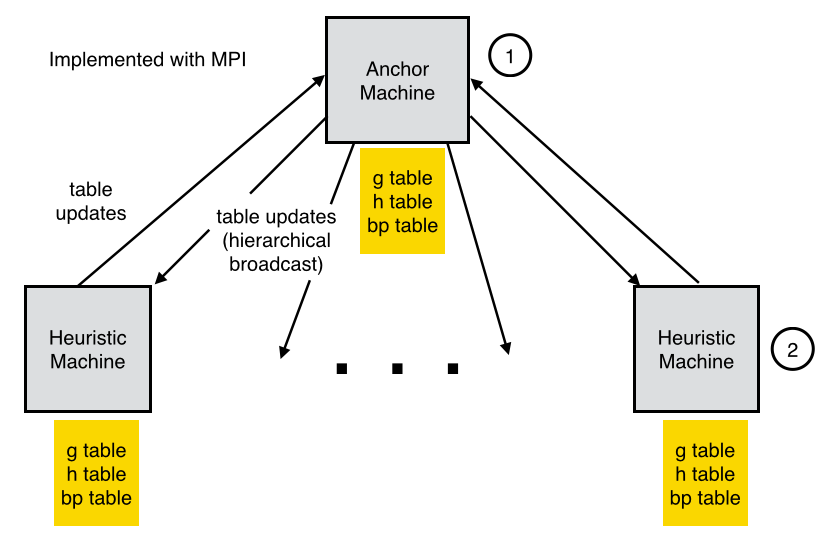
\includegraphics[width=5.0in]{system-diagram}
\caption{A diagram of our system. One machine starts up the others and runs the admissible anchor search. The other machines run their individual heuristics. Communication is done using MPI. 
\textcircled{1}\textbf{Anchor:} Starts heuristic machines; performs state expansions using anchor heuristic; receives, resolves, and broadcasts table updates; checks for termination conditions. \textcircled{2}\textbf{Heuristic:} Expands likely state (chosen using heuristic); updates path cost to its successors; communicate updates to anchor; termination conditions}

\end{figure}

\section{Experimental Setup}


%\section{Goals}

%\subsection{75\% Goal}
%\begin{enumerate}
%\item Implement parallel versions of IMHA* and SMHA*
%\item Identify bottlenecks in performance in running SMHA*
%\end{enumerate}

%\subsection{100\% Goal}
%\begin{enumerate}
%\item Implement distributed versions of IMHA* and SMHA*, perhaps with fancier distributed heuristic selection (there exists recent work which uses a simple form of online learning)
%\end{enumerate}

%\subsection{125\% Goal}
%\begin{enumerate}
%\item Design and implement a more sophisticated intermediate between IMHA* and SMHA*, based on the analysis of parallel and distributed system tradeoffs from our preliminary evaluations.
%\end{enumerate}


%\section{Resources Needed}

%We will probably need a machine with at least 32 cores for the 75\% goal and a cluster of some number of machines for the distributed version (100\% goal). We will be using MPI for message-passing between computers and C++ to program.


%\section{Relevance to the Class}

%We will investigate ways to parallelize SMHA*, and compare its performance to parallelized IMHA*. This project gives us the opportunity to explore classic tradeoffs in designing a distributed system, particularly between network latency and local computation.


%\section{Work Distribution}

%Tasks for 75\% goal:
%\begin{enumerate}
%\item Implement IMHA* using locks / shared memory
%\item Implement SMHA* using locks / shared memory
%\item Pull problem and heuristics from cited work
%\item Run algorithms on at least one of the cited example problems
%\item Evaluate performance overhead of the parallelism
%\end{enumerate}

%Tasks for 100\% goal:
%\begin{enumerate}
%\item Implement IMHA*/SHMA* using message passing
%\item Run algorithms on a cluster of machines
%\item Evaluate performance overhead of local and networked message passing
%\item Reflect and compare against multicore version
%\end{enumerate}

%Tasks for 125\% goal:
%\begin{enumerate}
%\item Implement new version of SMHA* based on considerations of the evaluation
%\item Test and evaluate
%\end{enumerate}
%\newpage

%\section{Final Paper Outline}

%\subsection{Introduction}

%Similar to the above problem statement.

%\subsection{Related Work}

%\cite{Aine14} (MHA*) presents the original multi-heuristic anchored search. \cite{Phillips14} (parallelized A* for slow expansions) presents a criterion for parallel expansion using locks, while retaining the approximate suboptimality guarantees of sequential wA*.

%\subsection{System Description}

%A distributed system running one heuristic on each machine.

%\subsection{Evaluation}

%\textbf{IMHA* experiment:}

%We will implement IMHA* on 32 cores, each running its own heuristic.

%\textbf{SMHA* experiment:}

%We will implement SMHA* on 32 cores, each running its own heuristic and updating shared data structures for path costs.

%We want to keep the approximate optimality guarantees of unparallelized MHA*, so this requires careful maintenance of the data structures to ensure the invariants are kept.

%Explore different way of updating the shared data (i.e. data replication and consistency checking/message-passing?)?

%Performance of the various implementations will be evaluated on the problems from Aine et al.:
%\begin{enumerate}
%\item Robot arm manipulation
%\item 3D path planning (navigation)
%\item Sliding tile puzzle
%\end{enumerate}

\subsection{Conclusions and Future Work}

\bibliographystyle{ieeetr}
\bibliography{sources}


\end{document}